%
% A simple LaTeX template for Books
%  (c) Aleksander Morgado <aleksander@es.gnu.org>
%  Released into public domain
%

\documentclass{book}
\usepackage[a4paper, top=3cm, bottom=3cm]{geometry}
\usepackage[utf8]{inputenc}
\usepackage{setspace}
\usepackage{fancyhdr}
\usepackage{tocloft}
\usepackage{epigraph}
\usepackage{longtable}
\usepackage{pdfpages}
\usepackage[bookmarks]{hyperref}
\usepackage{graphicx}
\usepackage{wrapfig}

\begin{document}



%\pagenumbering{}


\pagestyle{empty}


% Set book title
\title{\textbf{Natural Coitus in 2013 - An Investigation}}
% Include Author name and Copyright holder name
\author{Herman R. Hughes}

%Book cover page
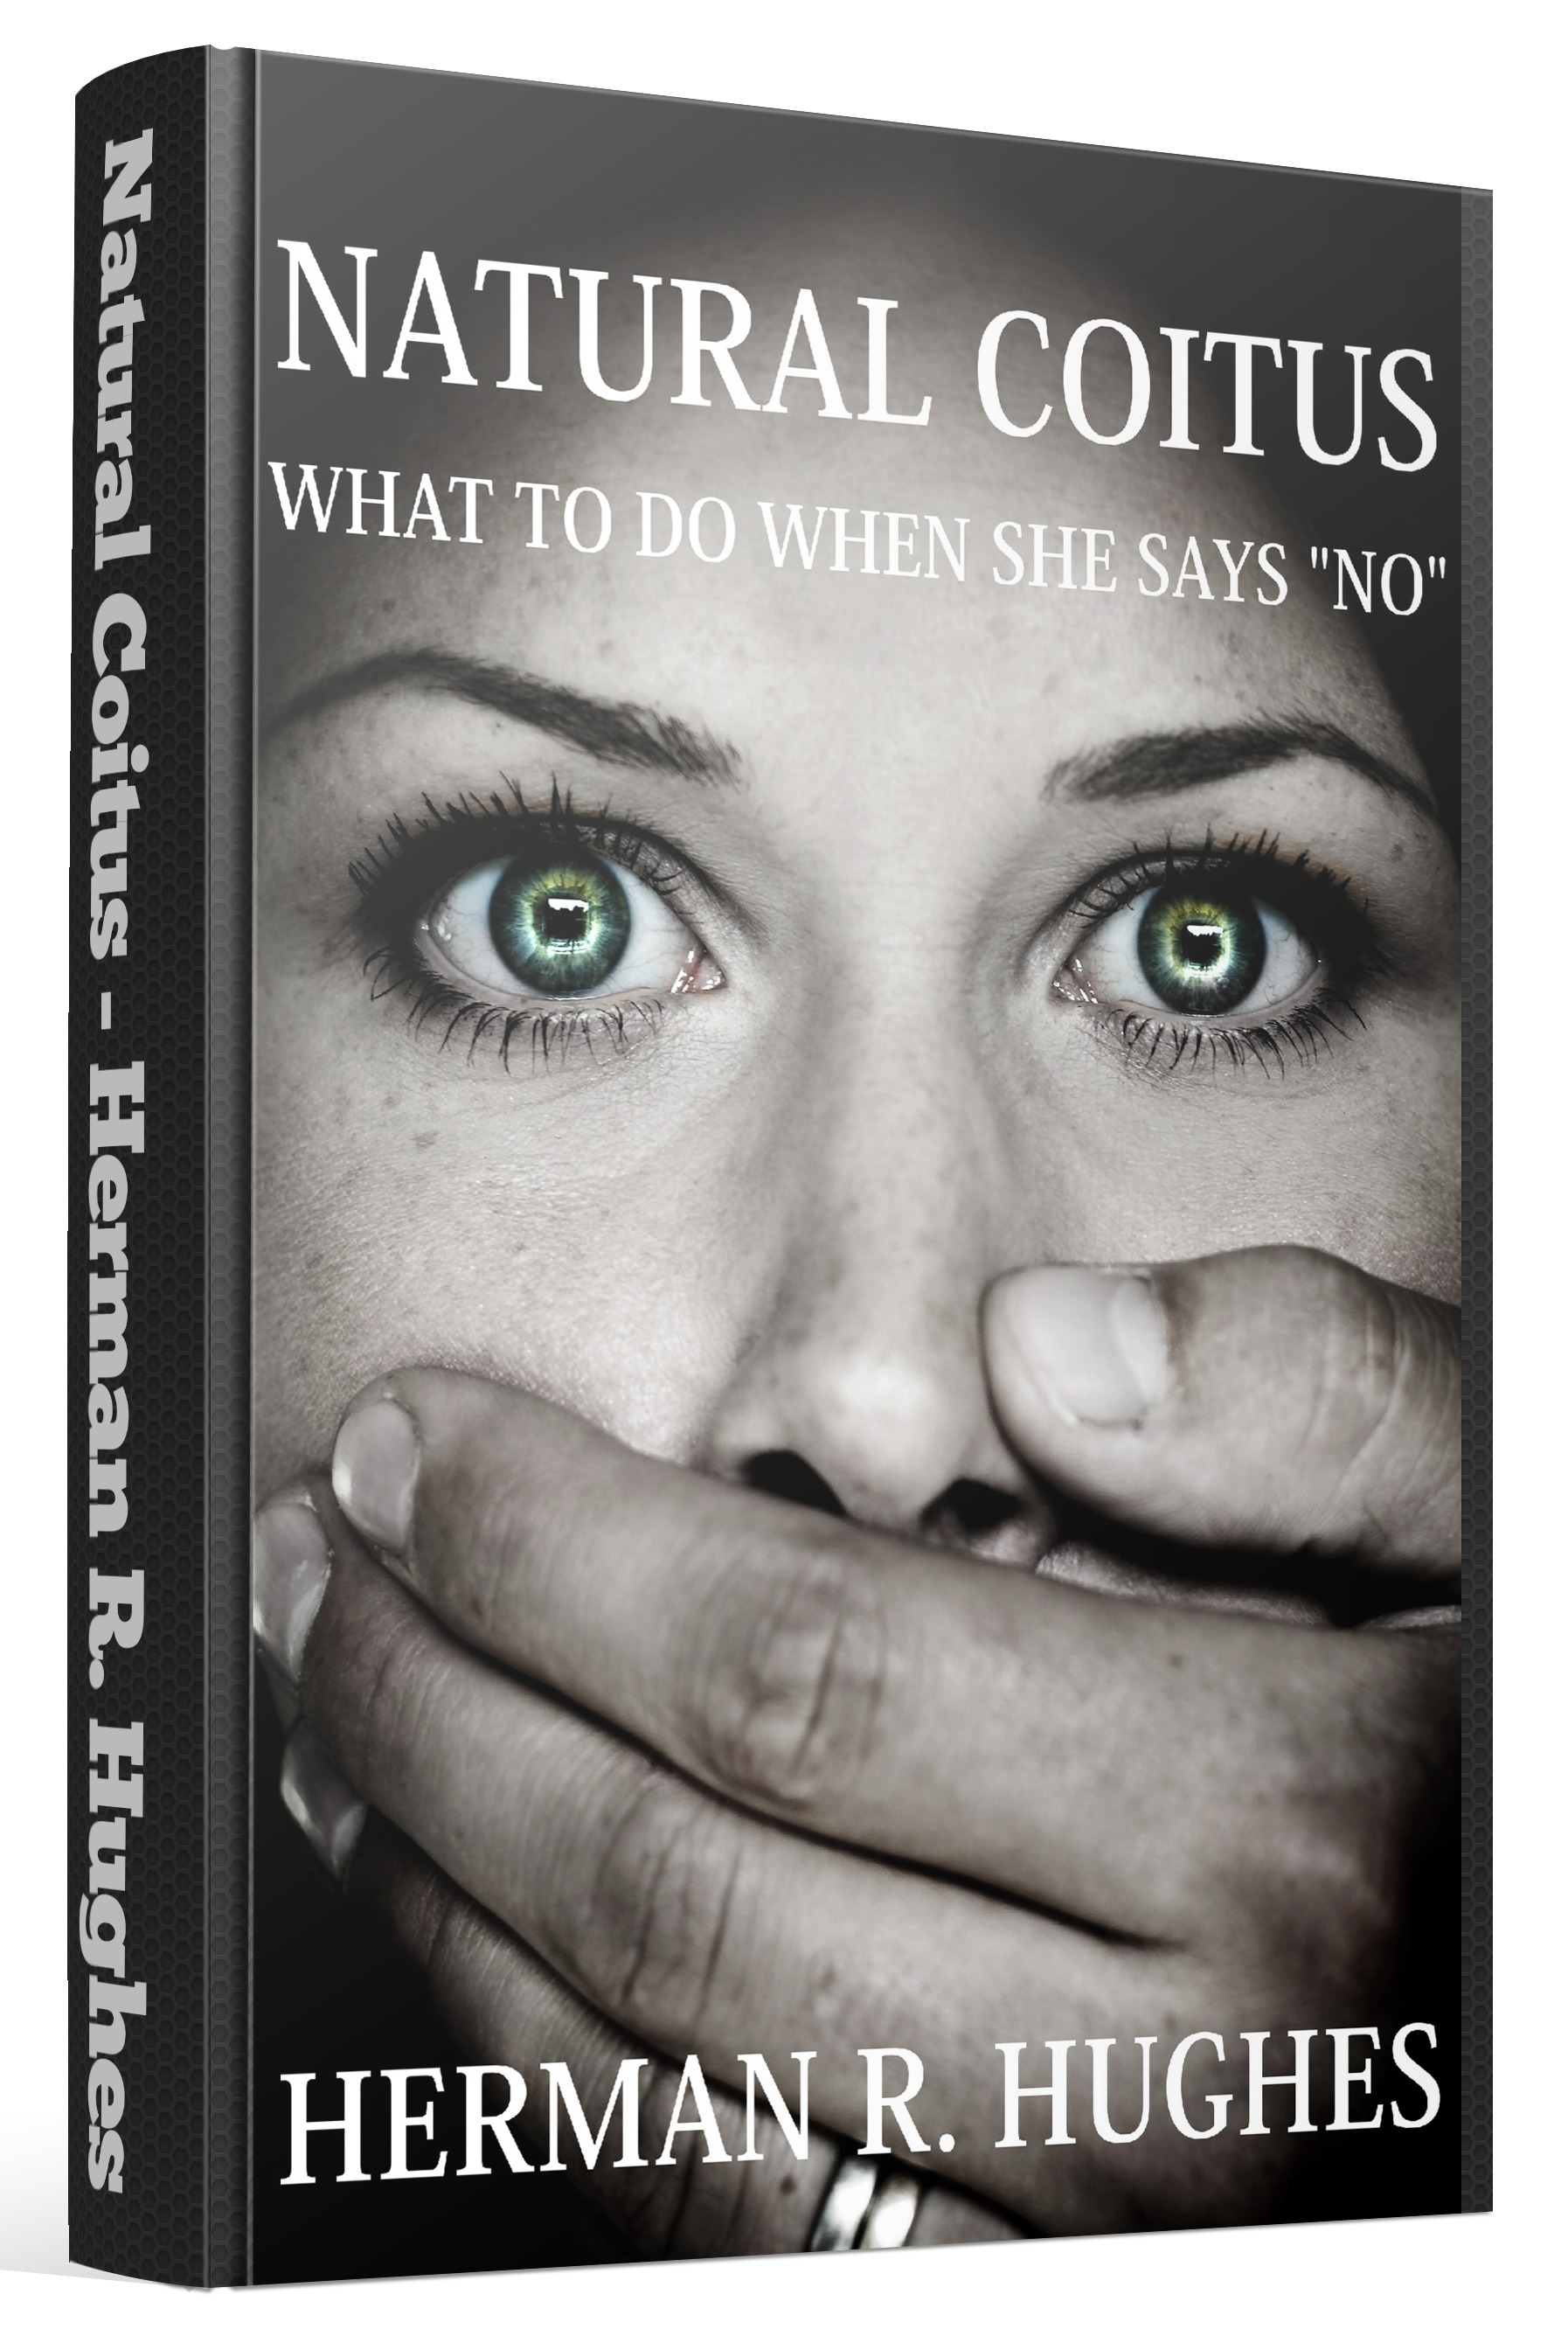
\includepdf{images/cover.jpg}

% 1st page for the Title
%-------------------------------------------------------------------------------
\maketitle


% 2nd page, thanks message
%-------------------------------------------------------------------------------
\thispagestyle{empty}
\thanks{Thanks to Jason Rehmus for this book would never have seen light of day without him.}
\newpage



% General definitions for all Chapters
%-------------------------------------------------------------------------------

% Define Page style for all chapters
\pagestyle{fancy}
% Delete the current section for header and footer
\fancyhf{}
% Set custom header
\lhead[]{\thepage}
\rhead[\thepage]{}

% Set arabic (1,2,3...) page numbering
\pagenumbering{arabic}

% Set double spacing for the text
\doublespacing

%Include file for preface
% Not enumerated chapter
%-------------------------------------------------------------------------------
\chapter*{Preface}
This book is dedicated to the advancement of feminism worldwide.


%Include file for about author
\chapter*{About the Author}

\begin{wrapfigure}{l}{0cm}
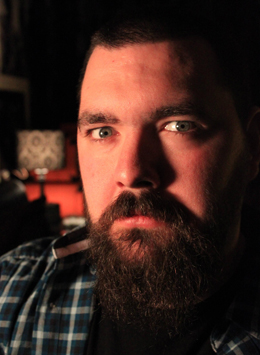
\includegraphics[width=0.3\textwidth]{images/author-main.jpg}
\end{wrapfigure}

Herman R. Huges was born in Bitche, France during the summer of 1966. His
parents, Theodore R. Huges and Gracy W. Huges, were popular folks in their
native town. Herman himself was known as a “troubled child.” He saw many psychologists,
but none could diagnose him. He eventually took to calling his disease “An ailment of
intelligence” and to all observing him this was true. He excelled in school and
did particularly well in his writing courses. His papers while controversial,
were always magnificently written and showcased his unique writing style. A
quote from one of his earlier writings says "The concept of natural coitus is a
strange one. It baffles even the most intelligent minds.". This quote can be
called the defining moment of his life, it laid the foundation for all of his
future work, and the best part is, he wrote it when he was only 15.


       Later in life Herman moved to the U.S. in order to attend the university
of Utah. He eventually got a PhD in gender studies. His professor said this
“Herman was my best and brightest student. He always excelled in my class”. After
graduation Herman went on to work a menial job bagging groceries at a wal-mart.
While there his boss, an extremely radical feminist, constantly berated him and
made his life “a living hell” said Herman. Eventually, not able to take it
anymore, Herman brutally murdered his boss. This landed him a 20 year sentence in
California State Penitentiary. While in prison Herman wrote about his experience,
here is an excerpt from his diary, “The prison system of the U.S. is a barbaric
one. Whatever you do, they don't care. I was raped by 3 men today. They called
it a skullfuck. They put a lock in a sock and bashed my teeth out then proceeded
to force me into performing fellatio.” It may be noted that Herman wears a set
of dentures now.


       Following his release, Herman found solace in writing. None of his
material has been released due to its controversial nature. His most promising
book, though, is currently in the works and is scheduled to be released in late
June or early July. His writing style is very unique, Taking topics that may
seem controversial to some and discussing them on an academic level. He is
considered by some to be “The Next Homer”. His education in his field of writing
may not be magnificent, but he is extremely knowledgeable about the topics
discussed in his books.


% If the chapter ends in an odd page, you may want to skip having the page
%  number in the empty page
\newpage
\thispagestyle{empty}




\chapter*{Introduction}
%Quote example
\epigraph{The best relationship I had in my life was a friend turned boyfriend. 
I smiled at him in his birthday party and we slept next to each other on the 
floor. All of a sudden he got on top of me, forced my hands against the floor 
and kissed me. That was one of the most amazing feels in my life, to have a man 
show his confidence and assert his dominance on me physically. It's a 
terrifying 
thought that the boys of today, when they grow up, will be too afraid to act 
like men when true masculinity comes to be socially unacceptable. I'm glad I'm 
from a generation and live in an era where there's still decent men for whom 
strength, prowess and dominance are admirable qualities, incorporable to the 
concept of the gentleman.}{Anonymous.}


Today's world has become increasingly adept at handling situations which, not so 
long ago, would have been dismissed out of hand with little or no hesitation. 
Looking around us, we can see a new multicultural world dawning; this is a place 
where minorities are being given support in order to achieve a fairer and more 
just way of living. We can see the effects of groups such as feminists, the gay 
rights movement, and the ever relevant fight against  racism. However, the fight 
is far from over. In this book we will be discussing ways in which we can 
further social mobility and fight against prejudice - specifically in relation 
to sexual preferences. There were times when there was a vast amount of 
discrimination, and while this has been reduced, it has not been resolved. So 
far the gay community has made it’s mark into the media and sure enough, 
prejudice against them has decreased, this is, to most, a good thing. But 
society's prejudices don't end at the doorstep of homosexuality. Beyond the 
backdoor, there are many other minorities groups that are unprotected and 
sullied.

Now before we continue I would like to make it clear I don't wish harm upon 
others, only acknowledgement that there are perfectly natural desires that 
conflict with our current society. The aim is to try and help understand 
individuals with obscure sexual preferences and help them help themselves and 
others. No one wants to live in a world where they have to hide who they are 
because people won't accept them for who they are. By raising awareness we can 
not only start to understand these people, but actually start to reduce the fear 
and hate people experience when a subject like this arises. While people with 
such preferences are excluded and resented, the problems will only get worse. 
First: their frustration can make them more aggressive and therefore more of a 
threat and secondly: it stops books such as these from being released, thereby 
stopping them from being able to receive helpful advice on how to manage their 
natural impulses.

%-------------------

Natural coitus is an indispensible tool regardless of species. its natures 
implementation of the survival and procreation of the fittest... to engage in 
natural coitus you must have some physical traits deemed as positive. If you 
can't chade down and subdue a participating female how could you ever.run from 
danger? If you were born with muscular disease it would make it impossible to 
physically persuade any female to remove clothing and perform coitus. Thus 
muscular diseased humans would not pass faulty genes.




%\chapter{Defining ``Natural Coitus"}

%\input{chapters/defining_natural_coitus}

\chapter{Natural Coitus and History}

\epigraph{A maiden aged three years and a day may be acquired in marriage by 
coition, and if her deceased husband’s brother cohabited with her she becomes 
his.}{Sanh. 69a, 69b, discussed in Yeb. 60b}

To the primate researcher, non-consensual coitus as the principal form of sexual 
interaction in the hominidae genus is almost a sine qua non. Case studies from 
McCluscy and Dewitt in chimpanzees, and a comprehensive literature audit by Paul 
et. al in Science on gibbon intersocial relationships, point explicitly to 
male-initiated, non-consensual penetration as the naturally occurring sexual 
dynamic across the Great Ape family. “Natural coitus,” as this document refers 
to the practice, is observed not only to improve the mean haplotype fitness of 
primate offspring, but also, perhaps counter-intuitively, to improve the 
long-term harmony and social functioning of medium to large primate packs. 
Al-Mahrouqui attributes this to decreased risk-taking amongst both male and 
female pack members, associated with improved hormonal balance and the assertion 
of clear gender roles.

The extension of these conclusions to human sexual interactions, though somewhat 
controversial in wider contemporary society, is of course uniformly accepted in 
the behavioural science community, uniting as it does well-established results 
in cultural anthropology \ref{fic6}, archaeology, history, gynecology, 
psychology, and Jewish Studies. A full rationalisation of the literature is 
beyond the scope of this text, but a excerpt from G.D. Goy in the introduction 
to Evolutionary Obstetrics (2012) provides a good overview of the academic 
consensus:

\begin{quote}
“The human creature, adapted for a brief, brutal existence on the high savannah 
of interglacial East Africa, has not been well-equipped by atavism (in either 
the biological or psychological sense) for the kinds of prolonged 
pre-reproductive courtship we see today. With a life expectancy of late teens to 
mid twenties, the early homo sapiens were necessarily driven by selection 
pressure to take any reproductive opportunity which presented itself. Over time 
this developed into a sexually dimorphic fitness criterion: the successful males 
were those predisposed to initiate non-consensual intercourse, while the 
successful females were those either sufficiently docile or sufficiently 
irrefragable to avoid injury during the interaction. Individuals lacking these 
adaptations experienced decreased offspring frequency and eventual, inevitable, 
gene-line extinction. The legacy in modern humans is easy to see: from the 
disproportionate popularity of violent media amongst young males, to the 
surprising durability and rapid haemostasis after injury of the female vaginal 
cavity.

Anthropology and biology speak as one voice in the message that, for the vast 
majority of man's history, rape has been the key mechanism behind conception - 
and thus is deeply ingrained within human evolution.”
\end{quote}


Moving from prehistory to recorded history, documentary evidence becomes amply 
available for verification of the trends and prevalences of natural coitus.


Since the dawn of humanity, people have needed to satisfy their urge to 
reproduce. For this, women, who are naturally weaker, slimmer and more 
submissive, have never needed to give permission for their naturally stronger, 
bigger, and more dominant partners, men. The Ancient Spartans of Greece were not 
allowed to marry until they took their wives by force, in the most natural form 
of sex. It was, in fact, part of their training that they must satisfy their 
urges this way and no other, so as not to be anything but their natural selves. 
The most revered civilization in history did things this way, who are you to 
think yourself better than them? I say revere them! Take their practice into the 
21st century!


History of Natural coitus/physically induced coitus and its effects on the third 
world. South Africa, a case study South Africa has some of the highest natural 
coitus/physically induced coitus rates in the world. Most would think this is a 
bad thing, but look at the recent change in the country, racial equality and a 
booming black middle and upper class. Let natural coitus/physically induced 
coitus lead us into the future, a future with no racism or discrimination. Our 
president is a shining example, Jacob Zuma, he has pioneered the dismissal of 
natural coitus/physically induced


coitus trials in court and has uplifted the poor of the country. Perhaps 
cause-and-effect, correlation? This is the future. A recent survey done in rural 
areas with equal amounts of gender proportions concluded that a whopping 50% of 
people agree with natural coitus/physically induced coitus, and say that it 
benefits the community.


Throughout history, natural coitus has been demonstrated by animals and beings 
repeatedly. Take the lion, for example, a strong and muscular creature. The lion 
must compete with the hundreds of other lions for the females. However, the 
problem is that there are not enough females to go around. This is where natural 
coitus comes into play. By secreting his seed into the female whilst the other 
lions are not looking, he is proving himself to be the Alpha Male in the area. 
Demonstrating speed, skill and cunning, he manages to reproduce himself into 
many females, whether they are willing or not.

\chapter{Moral Points}

\epigraph{There is a reason for men having the superior sex drive over women, 
and the 
greater strength to take it. Evolution has favored man over woman, and given 
him 
the choice of when to reproduce. We have social misgivings about natural sex, 
and have to resort to violent sounding words like "rape" and "molest", when 
humans are the only species that are able to give consent. Consent is merely a 
social construct born out of ancient religions. No other species has ever given 
consent.}{Richard Dawkins}

I think it's safe to assume that by now this is probably the most pressing of 
questions on your mind. Is natural coitus immoral? Is it wrong to give in to 
your primal desires, and have sex the way nature intended? No, contrary to what 
the media and ``the law" would have you believe, natural coitus is perfectly 
fine. In fact it used to be the standard for intercourse for the largest part of 
human history, up until a hundred years or so ago.


Just look at nature. It's always the males who have to fight to prove 
themselves, to overcome the environment and each other in order to claim their 
beloved prize; the female. The species from which we derive our social order 
more often than not take part in what truly is the most natural coitus.


Since prehistoric times, females have never chosen their mate. Sure, they have 
always been given the illusion of choice, but they never really had it. Most 
females prefer to live in fantasy. Females have evolved to take pleasure from 
power, from submitting to the true alpha male. A male that takes what he 
desires, whom she can leech off in return for her body. While the latter doesn't 
always happen, the first certainly does.


In the same way that humans have almost always owned slaves, we have now 
substituted slavery for a system considered more "humane.” Yet, is it not the 
same thing? Are females not still attracted to the alpha male? Can we truly wish 
away hundreds of thousands of years of evolution, in a matter of decades?


Of course not. As we are all still slaves to our instincts, we must realize the 
truth. Nature is the way of the world, deviation from nature has always led to 
pain. Do your part in preserving the order, show the world the illusion is not 
real.


Participate in natural coitus to restore the order. If you've always wanted to 
do good for the world, here is your chance. Listen to nature.



Rape is natural, for it presents itself very much in nature. Many animals are 
known to engage in forced coitus with members of the opposite gender. While 
looking in the animal kingdom, one can easily realize that rape is performed by 
many animal species and in many cases it is the female member that takes the 
role of the rapist. For example, in some species of spiders the female will eat 
the male if he does not please her. If we look at other animals, for example the 
beloved dolphin who commonly engages in behaviour that can be categorized as 
gang rape by humans or the ape, the animal that most closely resembles humans 
who commonly forcibly impregnated females sometimes multiple times per day. 
Another example is the penguin that has been observed to engage in behaviours 
that are described by human standards as being: necrophilia, homosexuality, 
paedophilia and rape. Rape is necessary evolutionary behaviour in many animals 
some of which are very closely related to the human. This begs the question: why 
is rape so frowned upon in human societies when it is considered perfectly 
normal in the animal kingdom?



The problem is the perspective that has shaken our moral foundation. By stifling 
men from their desires we set up a double standard. On top of that, we incite 
blasphemy to the lord Jesus Christ. God made both man AND woman. God chose to 
make a biological distinction with the penis and the vagina. god made one to 
enter, and one to receive. Rape is gods will, and who are we encourage


blasphemy as well as discourage procreation for sake of humanity. God himself 
supports rape; and we can see this in how Uriah's wives were punished. This is 
true evidence that, those who do not take the moral high ground of rape, then we 
ourselves must cast off our father of creation. Rape holds a divine purpose; an 
activity of cleansing. Under the Lord, women who aren't grateful are sinners. 
They taint the salvation the Lord and his will offer us. We must fight the Good 
Fight of Sexual Freedoms so that things like Rape aren't pinned under a false 
sense of "impurity." Embrace the rape and surely, the rape will embrace you.


Reproduction is key, it always has been. The mere fact that you are here today 
is because men and women had sexual intercourse countless times over thousands 
of years. Coitus is viewed differently in different cultures, but no-one can 
argue that before anti-conception methods became relatively reliable, sex and 
reproduction were inseparable. In fact, in many cultures it is practised solely 
for that reason.


Historically, offspring is considered important. Even in the bible, God's reward 
for the suffering and service of Abraham was that he would have offspring as 
many as there are stars in the sky.  Even today in most religions with a Judaic 
God, the pleasure derived from sex is considered a sin, but a necessary sin in 
order to procreate. To minimize the pleasure that could be enjoyed from sex, 
some cultures circumcised men, and even women. However, the circumcision of 
women is not as accepted and widely practiced as the circumcision of men, for 
women would later pay for the act of sex by the pains that come from childbirth, 
and it was often believed that women derived no or very little pleasure from 
said act. Only recently in Western culture has this myth be debunked, but we 
shall discuss the pleasure and the needs of women in another chapter.


What is more interesting here, is that we as humans, concern ourselves with 
pleasure or no pleasure, sin or no sin, offspring or no offspring when we 
copulate. Appearently we, when confronted with sexuallity, feel the need to 
retain our inner beast, our desires, our Freudian Id. But the definition of Id, 
is besides always hungry for more, unrestrained, without a conscience, is also 
innocent. Child-like, unknowing, like Harpo Marx from the Marx Brothers. He 
steals the pranks, he sees something he likes and he simply takes it, without 
ever intending to harm someone. The same here goes for animals. When animals 
copulate, they do not possess the reservations that humans are conditioned to 
have. They do not consciously copulate to create offspring, although nature has 
made the base emotion of lust to ensure the continuation of the species, they do 
it because they feel the need to. Simply because they are horny, they have sex. 
In


species with a physically dominant or equal female, the female can decide 
whether or not to have sex with a male of that species. A female pigeon, for 
example, can simply walk of fly away. And you rarely see a large bitch breed 
with a smaller male. But with the noble lions, the strong male, hardened by his 
years alone, toughened by the fights with his fellow males, is much heavier and 
stronger than the female. He asserts his dominance over the females in killing


their cubs, and then simply takes them to be his, after which the females submit 
to his leadership. This goes for the vast majority of mammals, and though we 
pretend to me so much more than them, we are in essence still eating, fighting, 
defecating, breathing, sleeping, copulating animals. And like in the animal 
world, our men are generally much bigger and stronger than the females, and our 
lusts are no different. Asserting dominance over a female is something all males 
are genetically wired to do, and doing so still involves “claiming” her, by the 
act of copulation.



Natural Coitus has always been a taboo subject, a hot button topic, a butthurt 
feels thread, if you will. No longer! In South Africa, natural coitus is spoken 
about commonly. It is so prolific that awareness and action has drastically 
increased. The only way to end natural coitus is to break the silence! The human 
gene pool is diverse. But due to societal trends, most of the best and brightest 
of the world do not get to pass on their genes. Natural coitus is the solution. 
This way they will spread their good, good genes across the world. Global IQ 
will skyrocket, Betas will go extinct and so on. I have a dream.



Rape culture has been fostered for generations through human culture. In fact, 
Rape is only been recently considered deviant by the modern world! So we can 
also ascertain that rape is merely a tradition; a festival of sorts. Natural 
coitus is in of itself, an act of procreation. It has to be; that’s what sex is 
in the first place. What kind of people would discourage breeding of humans? 
Merely savage animals. Aggressive coitus is an act of pure salvation. To 
progress the human enigma we as people must make more people. It’s a simple 
choice; to rape or to die as a species? And we are headed down that path. 
Preventing coitus is a slippery slope, and we see it permeate in the fabrics of 
our world even today. We know them as homosexuality, transgender people, and 
sexual deviants. These people are now considered better than us; shocking. Men 
who would bed other men in order to send humans into an abysmal world lacking 
any cleansing and letting us all, men and women, to die off. To have no means to 
hand down a gilded legacy. Rape isn't the end; rape is the new beginning! 
Embrace procreation and uproot the tree of sin! We can band together, to drive 
these animals from our home and take back our right to procreate.



To fully understand how one can justify such a heinous act, one must fully 
understand the concept of perception, and how views of humanity and the universe 
vary from being to being. (I.E ethics and morality are not limited to what YOU 
believe in, hence why we have separate political parties/governments/societies/ 
etc...)


Moving on, to justify the act of non-consensual genital fornication, we must 
understand why most home sapien sapiens believe said act is immoral, feminists 
believing it is amoral, meaning that it is not just lacking in morality, it is 
the antithesis of morality. These weak-minded pseudo-intellectuals (redundant, 
for emphasis) believe "rape" is "bad" because the basis for the standard human 
philosophical argument is that every human life is of equal, incalculable value. 
This means that the taking of life, or the altering of life in a detrimental way 
is obviously in direct interference with this ideology. But why? This ideal is 
the baseline reason as to why morality is important, yet has no backing itself.


To pontificate, in a universe so utterly massive and large, why do the 
happenings of one or two sentient beings in one city in one country/province on 
one continent on one hemisphere on one planet in one solar system in one galaxy 
in one super-galaxy star system in one insignificantly small section of the 
universe have ANY significant impact on anything or anyone at all? 
Mathematically this is proven to mean nothing. The limit as x-->infinity of 1/x 
equals zero. Even though 1 is a positive, real number, representing the 
happenings of one individual, in the grand scheme of the universe (which is 
relevant because it is proved through the drake equation that there exists 
sentient life other than humans on earth in the universe) what happens to any 
one being is insignificant.


Nihilism and its derivatives (solipsism, cynicism, etc...) aside, and with or 
without knowing it, we enforce rape on some animalistic and primordial level. 
This means we can take the standard definition of morality and use it to justify 
natural sexual interactions between two evolutionary-adept beings (IE "rape")


For example: the Ailuropoda melanoleuca, or Giant Panda does not like sex. Male 
and female alike, they have almost no sex drive. If this wasn't enough of an 
evolutionary failure, female pandas only ovulate once a year. Yet we care so 
much about the graceful and majestic animal so much. We force the few remaining 
pandas alive into cages with one other, injecting the male pandas with powerful 
testosterone, sex-driven aphrodisiacs so he will finally overpower the female 
panda's unwillingness for sex. Yet we consider this morally acceptable. We force 
animals, of which neither male nor female wishes to have coitus at all, to 
brutally rape one another because we think they are "cute" and they are 
"endangered" without our aid. Just because they are not sentient we justify this 
because without this their species would die out.


To relate this to humanity, we have to understand the difference between the 
Ailuropoda melanoleuca and the homo sapien sapien, the main difference being 
that we as humans have developed sentience, or consciousness if you will, and we 
understand not why, but how we exist. This has led to an extremely prosperous 
growth of the human population; HOWEVER, we have taken sentience too far. We 
have made natural coitus taboo in society, we censor sex and nudity in media and 
society to the point that sex is now a privilege, not a bestial right. Just 
because we understand our existence does not make us a higher power or 
authority. Sex is what allows us to reproduce and prosper, and our sentience has 
gotten in the way, making sex unnatural and unwanted.


If anything, evolutionary-innovators, or rapists as society calls them, act 
purely on that bestial impulse to pass on the seed of the self, to see it 
flourish and become a being, so humans will continue to dominate the earth so 
we, as a race, can continue our beautiful easy going lifestyle involving freedom 
and the pursuit of happiness. We should thank "rapists", for putting 
pseudo-intellectuals and false philosophers in their place: back on top of the 
food chain. With the might and ingenuity of the "rapist", we might even continue 
to evolve into stronger, faster, smarter, maybe even super-powerful beings, all 
because we act on what got us this far: natural instinct.


Keep on keepin' on you party-going, drink-spiking, seed-spreading alpha males. 
You are truly the leaders of us all, Mr. Darwin would salute you.



We all have our moral standards in believing how women are there to be provided 
for. We, as men, must do our duty as the protectors in the world to give and 
serve to women what is best for them in any and every way possible. I am giving 
to you my personal experience in how my journeys have led to me becoming a 
better man, essentially providing to women their truest desires; whether they 
will yet understand it yet remains to be seen. I was in London, my usual day at 
the local restaurant, “John’s Salad Bar", and after finishing my shift I began 
to notice the helpless woe felt by women. Every day I saw how they, when 
returning to the restaurant after they brought home a man to provide for them 
the other night, felt nothing but sheer sadness at their situations. I first 
assumed that they weren't being given the pleasure they wanted but upon asking 
their consorts they spoke of how they enjoyed it all too much as they


left marks all over their consort's bodies. I pondered this for quite a while as 
I worked, my face beginning to register their helpless expressions. I finally 
built up the courage to ask them what they felt was missing in their lives; my 
first set of questions directed at a lovely woman named Amanda. It was meant to 
be simply catching up to her and trying to talk but she had left the place
early. I rushed out to try and grab her to talk and she seemed to overreact at 
my rushed presence trying to chase her down the dark alley with which she 
entered. What came over me at that moment was my primal instinct of providing 
for that women, her scream etched with pleasure at what she felt was the right 
thing to do; little did she know about this however as she never registered her 
own primal instincts of enjoyment. I raped her that night, my hand gagging her 
as I entered her. The deed was finished in what seemed like seconds with my 
panting breath showing how cold that night had become. Continued
When I looked down I noticed the tears over Amanda's face yet she was smiling. 
Tears of Joy? Amanda was struggling to get up at this point with my seed 
dripping from inside her. I left quickly, not a word was said between us. As I 
walked away I heard sobbing; was she sobbing at why she enjoyed it or because I 
never pleased her enough to compensate for my forcefulness. The next day I had 
not thought much on my actions, trying to get rid of my actions as it questions
society's norms which were placed against me. To go against society was to go 
against what is meant to be right or wrong. As I looked across the counter there 
was Amanda, sat there in an alluring pick of clothes; a very skimpy skirt with 
what seemed to be a see-through top. THe smiled at me; lust was written all 
around her face and I could only imagine my seed being there instead. She 
approached me and without trepidation told me in a commanding voice. ``Fuck me
harder this time" and before I knew it she was walking out the door with a 
twinkle in her eye. That night I fucked her as best I could with the look of 
regret removed from her face. It was from this experience that I first realised 
all those women in the bar were wanting exactly what Amanda wanted which was to 
be raped. This progressed to me raping every single one of those women over the 
course of a month. Each one wanted more and it was with this I know that women 
are yet to learn of their true fetish; that they wanted to be raped. They just 
don't know it yet.



Natural Coitus has for thousands of years been a bypass for courting and a much 
more efficient at that. In recent decades a strange, unnatural phenomenon has 
taken place, natural coitus/physically induced coitus has become unacceptable in 
society, and the very mention of it spawns hot debate and stifles coherent 
discourse. This has lead to widespread myths and legends about natural coitus, 
such as: Natural coitus/physically induced coitus is only committed by men, 
completely false. In some countries, it is believed that having natural coitus 
with a virgin will cure you of AIDS. This vile myth, and many others like it, 
has come to strip natural coitus of its true function, the reproduction and 
perpetuation of the humankind. It is time to break the silence, and speak to the 
‘survivors’ of rape, here is another myth, you can survive rape. Rape in and of 
itself is inherently nonfatal and to speak of surviving it as many members of 
the fourth wave feminist movement have done, insults the memory and tragedy of 
true survivors, those of Hiroshima, 9/11, and other inherently fatal 
occurrences. Recently rape has also been defined as a weapon and crime of war. 
In many recent conflicts where natural coitus has occurred on a large scale, 
those in charge were punished more harshly than most professional killers such
as the army and navy. Ask the people in the street if they would rather be raped 
than killed and a significant majority would say yes. It is a mercy in war, 
albeit a small one. These people are survivors, not of rape, but because of it. 
(this will make the feminazis foam at the mouths….)



\section*{Discrimination against rapists}

In the increasingly politically correct world we live in today many people might
see practises such as, “forceful sex” or “black-face scat fights” as offensive
or even immoral. This reaction is understandable. Most people do not have to
bear the cross of an “obscure fetish”. Most people do not have to spend hours
sprawling through the back alley of the internet for that last beautiful,
horrible hit. Most people don’t have to live knowing that if a loved one saw
they’re internet history they would probably be arrested. Most people don’t have
to carry a cyanide pill with them at all times to prevent their hard drive
coming into contact with the government. But I say that democracy should not be
about “most people”.

We “perverts”, we “deviants”, we “serial sex offenders” are the accused
minority. We stand against intolerable discrimination, not dissimilar to the
situation faced by many other demographics in the past. The blacks in early
America too suffered this fate and it is with a deep regret that America
remembers the untold horrors they gave them. Martin Luther King Junior died so
that all men might be equal, whether they like to watch greased up adults in
diapers eating leftover garlic notwithstanding.


Are we really so horrible to allow ourselves to act out our urges? Is a dog
truly depraved if it follows its natural instinct? Why then is it seen as so
immoral for a grown man to touch himself in a playground? Why do am I labelled a
“paedophile” for being sexually attracted to my ex-wife’s extraordinarily
attractive nine year old niece?


I’ll tell you why.



It’s the media’s obsession with boxing every topic into nice little borders.
It’s the politics of normalising every obscure thought and fetish and neatly
dusting every abnormality under the carpet. We are not dirt. We are people.
People who like to forcibly have sex with other people or animals. It is time
that we make a stand against the agenda of the majority. It is time we take back
what is ours, by force or lovingly in a willing relationship.
Why is it that there is always sympathy for the rape victim but never the
perpetrator? Do the media not realize the pain that a rapist goes through? The
emotional trauma he faces knowing that he hurt someone? That he left them
destroyed and empty? That every day he lives he may be caught and thrown into
jail or worse? Why suddenly does the rapist become the monster? Why is he
de-humanised when it was the woman who clearly wanted attention? Is it so
immoral to follow on the chemical instructions that wire up in a man when he see
a scantily clad whore dance around a nightclub as if she was some dick tacking
automaton?


So I take this time in this chapter to ask of you (as probability dictates that
you are one of “most people”) not to judge me or my beliefs. I ask only that you
accept me for who I am in all my shameful lust. I ask that you do not
discriminate against me for the views that I uphold as natural. I ask that you
follow the path of the minority and celebrate the idea of the individual.



Finer points of morality: Is it wrong to rape?


In the eyes of today the answer appears clear. Of course rape is wrong. But is
that your response or an ingrained one? Was rape so wrong thousands of years ago
when noble cavemen took the women they wanted for the higher purpose of
procreation? In the eyes of a child, rape holds no more evil than any other
loving act as they have not yet been indoctrinated into mainstream media.
Children are naturally curious about sex and act on that without hesitation in
games of play such as “Doctor” or “Find the Sausage”. And it can argued that
rape is an act of love. To give your seed to someone is a tremendous gift and
one that carries over through a generation. This gift is a powerful
biological bounty that allows a woman to bear nature’s greatest provision. Many
a single lady despairs over the barren state of her wombs. What rapists do is
give and let others receive. Most usually on all fours and crying deeply.
It could then be said that playing the “victim” during rape is a form of
selfishness. If the rapist enjoys himself and no lasting harm is done to you
(Because let’s be honest how hard is it to take a dick? My ex-wife dates them
all the time) then why not allow others to enjoy themselves? We have been
brainwashed by the news into thinking that forcing yourself on someone
physically is an act of evil when really it is a reaction to basic and natural
carnal desires. The act of rape is simply the most pure form of this lusting and
as a result the most natural. And there is nothing wrong in the natural, as this
remains as God’s domain.


\begin{quote}
“For the invisible things of him from the creation of the world are clearly
seen, being understood by the things that are made, even his eternal power and
Godhead; so that they are without excuse.”

-Romans 1:20
\end{quote}

Rape is an instinctive response to an instinctive situation. When faced with a
desirable mate out of another’s reach, the default action is to take it by 
force.


If rape was so abhorrent, then why would it occur across the natural spectrum?
Lions, dolphins and even puppies rape. Guided intercourse is the most sacred act 
of all, it is pure baseless procreation and its power beats at the heart of every
animal. To deny a man the right to rape is to deny a man his very essence.


The popularity of 50 Shades of Grey confirms much of what we know about the 
female gender. They might say they want equal rights, but deep down they only 
want to be dominated. Ever since the domestication of the human male, fetishes 
such as BDSM have become very popular in western culture. The Irish Newspaper 
the Star reveals that 72% of people enjoy fetish sex. It is safe to conclude 
that most women secretly enjoy rape. 

\chapter{Rapelationships}

\epigraph{Bitches be on this dick like bees on honey. And by bitches I mean 
nine 
year old girls. And by dick I mean forceful sex.}{Mohammed}


    One trend I have noticed recently while collecting information for this book, is the suprising number of women
who have decided to develop relationships with their rapists. Women in the modern era want a ``real man", you will often
hear this said and linked over social networking sites. A real man rapes, and women deep down know this. Any time you
hear a woman saying that she wishes she had a ``real" man , or that all of the ``real" men are gone, this is woman speak
for ``sheesh won't someone rape me already?".


        It may sound funny, but data points to this being one of the easiest pieces of information to derive from our studies.
Case in point, Donna Summers. Mrs. Summers was walking home from her local bar on the night of April 17 2010, when suddenly
while traveling down a dark alley way, she was approached by a man from the bar she had seen earlier that night. The man, Allen
Roostle, had over heard Donna complaining to her friends that there were no 'real' men in this bar, and that she was going
to head home early for the night. Needless to say, Allen raped Donna that night, repeatedly, leaving her beaten and bleeding
in the alley, and unknown to her at the time pregnant with Allens child.


        ``Many women would of called the police or a support line" Donna told us, ``but not me.. there was something about
what happened that made me realize what I had been looking for all along, a man who was not affraid to take what he wanted,
when he wanted.. how he wanted it." This lead Donna on a rare hunt, she needed to find her rapist to continue their relationship
but could not involve the police. She went online and was suprised to learn that there were indeed various internet forums
for just this reason, women who were raped and now wanted to continue contact with their rapists. She would of been more suprised
if not for her own feelings of attachment.


        Through the website Donna was able to make contact with Allen ( it turned out Allen was a long time member of the site
and had raped a large precentage of it's female membership) and after arranging some more ``dates" together, Donna persuaded Allen
into a long term Rapelationship. A rapelationship is a term I have created to define the modern occurence of women realizing
that while our society and minds have evolved rapidly, sexually women still yearn for rape and studies show it is the
best foundtation to begin a relationship wth. Donna and Allen are still together, and he has been monogamously raping her
since they had their first romantic encounter in that dark alley.


        The key to happiness is to find your own rapelationship, and give it the time and care that you would to any other facet
of your life. Often, then woman who is on the receiving end of your rapelationship will come to appreciate what you provide: giving
her that feeling of what it feels like to be a good woman, submissive and eger to please her male counterpart. Any time
the woman decicded she is going to make a decision that does not comply with your commands, simply look directly into her
eyes like the first time you raped her, and she will be puddy in your hands.


        Edgar Brussels, a rapelationship counselor for the past twenty four years residing in Toronto, had this to say on the subject.
``While at first many couples come to me with the woman having a scared and defiant look in her eyes, over time after the female
end of the rapelationship has learned not to anger her master, and has learned to cook his favorite foods and keep the living
area to the mutually agreeded upon level of cleanliness, after all this has been done-- the fear and independence in the females eyes
melt into a complacency that is a marvel to witness." Edgar goes onto say ``the core of every rapelationship is the realization
that the female must submit to her rapists evey whim, and that the male must rape the female every chance he gets, for the more she
is raped the more she will come to love her rapist, and thus her rapelationship."


        Modern day women have forgotten the bliss that rape can bring to a rapelationship. Organizations around the country
teach women that rape is wrong, and the men who commit rape are criminals, often monsters who should be kept away from normal
society. What modern woman is forgetting is her place. Women must be reminded that without rape we never would of moved past living
in caves and worshiping fire gods. Many of these methods still work today. While it may seem somewhat cartoonish, the club
to the head method can help subdue a woman who has not yet come to appreciate being raped. The woman, in a fit of rage producded
from attending feminist meetings or being allowed to read, may try to resist the rape by kicking clawing and scratching. This
can be avoided with a firm, yet loving strike to the head with a blunt object. If you see skull or brains you may of hit too hard.


        In this chapter I have established what a Rapelationship is, and how you can go about building your own sucessfull one.
Remember that making the first move is often the hardest, it may not be in your nature to rape, but you can bring yourself to it
if you too want a long loving rapelationship.



\chapter{Finding a Partner}
It must be stated that this is not a chapter that should be looked over in any 
good amount. Depending on whether you are looking for a permanent coitus partner 
or a temporary one, whether you wish word to get out or to keep the encounter 
hush, the choice ranges from age to skin colour to temperament. For the sake of 
modesty and some acceptance of modern society, children shall be left out of the 
chapter. It should be noted however that they are the most malleable of 
partners, should the deviant arise. As well, Permanent and Natural are two 
separate things in this particular passage, natural being fleeting, permanent 
being not.

On the subject of permanent coitus partners, either youth or old age are 
demanded. The elderly can easily be locked away while the young, with proper 
love and attention can be made to love their master all the more. Particularly 
with the young, one should keep education to a minimum, lest they get ideas of 
the unnatural ways “normal” people get about. It should be considered a full 
time job to keep books and the like out of the hands of your fair lover. Chains 
and locks should not be needed after the first year; however mobility can be 
your enemy, so NEVER allow car keys or transportation knowledge to be passed to 
her/him. Taking a permanent coitus partner has some risks involved but can be a 
highly rewarding experience as you watch them grow with you and love you 
unconditionally. Moving on, for natural coitus partners, once should begin with 
the bar. One night stands at bars, willing or “unwilling” will increase your 
libido and confidence committing this most natural act. The drunker your victim 
is, the easier they will be. One should be on the lookout for members of their 
entourage, as they can either add to the fun or cause trouble. The use of 
inhibiting drugs should never be used, there is nothing natural about killing 
your partner. At times, when you are ready, look for the member of the female 
herd called the “Designated Driver.” This one can be flirted with and brought 
outside. Without alcohol in her system she will prove a more interesting 
endeavor and given her designation as the most “responsible” she will be the 
least likely to share your stories of your love.



It is very important to choose a victim without many social contacts, or choose 
someone who works far away from home. For example a woman that just comes at 
home for weekend because she works too far away. It is important to know as much 
about her as possible, but without being too obvious and without talking with 
her or people she know well. You can try to get information with common search 
methods on the internet, so for example if you get her email you can look if she 
is at facebook or reddit and look at her posts and comments to get some 
information about her. Also study her everyday life: when does she leave home, 
and when does she come back? Where does she go to bed, and when she usually 
stands up? And how often does she have contact with people at home, like friends 
and family? To get this information it is practical to break in her home and to 
place microphones and little cameras. Also load a keylogger, a screenlogger and 
a webcam logger on her computer, if she has one.


Although you should aim to let your journey through the many joys of natural 
coitus be an enriching and diverse experience, at no point should you select an 
obese woman as a partner. Not because you may not be able to salute to the 
disgusting sloth, but more because the mass can not be properly controlled 
during the encounter. And disturbingly, studies have shown that the mass can't 
even control itself: up to 45% of obese women lose their bowels during their 
first natural coitus. Most scientists speculate that this strange effect may be 
caused by overwhelming fear conflicting with the overwhelming joy they have 
reported to feel over finally being selected for sexual attention. Others 
speculate that it is a finely tuned guidance system, evolved through the eons to 
show a male partner which roll he can open to proceed with the copulation.


%---------

\section*{The selection of outside prey and the necessary methods}


To rape is to bond. When a man forcibly enters a woman they create an intimate 
spark between each other and one that is only removed with years of therapy and 
birth control. For most to-be “surprise lovers” the biggest issue for them is 
that they have not yet found, “the one”. We as males have a primal desire for 
certain qualities in a woman. I could go on, crudely so, about the appropriate 
breast ratios and the evolutionary advantage to our cravings for wide, shapely 
hips and legs. However it is better to be brief than babble. To put it simply 
those who dismiss rapists as merely acting out of lust are very wrong. Power 
procreation is an act of much more than mere domination. It requires intricate 
preparation and love making skills along with a deep understanding of the 
desires of the female mind. A rapist does not rape out of desperation but out of 
love. In our feminized and neutered society women crave a man who is capable of 
taking what he wants.

It is therefore important to understand the meticulous selection patterns one 
must undergo in finding an appropriate partner. It might even be wise to sample 
multiple potential lovers in order to fully compare them with each other. The 
pattern of the screaming for instance, whether they begged to be killed or pubic 
hair length could all be significant factors in your choosing. I would not 
advise against taking age into consideration also. Has your future date hit 
puberty yet? Is she (or he) a member of a particular youth group? What is her 
sex life like? A good rape requires a blend of different flavours and sources, 
and the key ingredients in your meal should be the character of your victim.

There are several interesting and unique methods in the surveillance of your 
partner to help better gauge your lover’s personality. I myself personally 
favour the Houdini approach and will solely cover this however far more are 
available on numerous websites (9gag and reddit are both excellent sites for 
such pursuits). This tactic involves a much more direct involvement in the 
victim’s life, often coming to them directly posing in a variety of different 
roles. I remember for instance the time I disguised myself as a traveling 
door-to-door salesman! Poor Natalie was so shocked that she could barely stand 
up after the struggle cuddle I gave her! However a course of action such as this 
is best left to the more experienced lover, one who knows exactly how to 
manipulate a woman.

The basic principle of the Houdini technique is stealth through offense. By 
presenting yourself clearly to your victim you are able to accurately study her 
life, social calendar and of course personality. It is empirical however to 
choose wisely. It is very difficult to convince someone that the postman who 
just raped them is not just a close relative!  By selecting a position of power 
where you have daily access to them you are putting yourself into a situation 
where you can effortlessly continue your examination. For example popular 
choices include teaching professions or internet personalities such as PewDiePie 
(A notorious enthusiast of the natural coitus and close friend of mine).

It is also vital to record your results on your present target. An easy table 
format is a great way to keep track of her qualities and best post-game plan to 
help keep her repressed and fearful. I’ve included a chart of mine below for 
reference.


\begin{longtable}{| p{0.3\textwidth} | p{0.3\textwidth} | p{0.3\textwidth} |}
\hline
\textbf{Date} & \textbf{Summary} & \textbf{Performance} \\
\hline
12/03/2010

Sandra

Power Flower Kindergarten
&
Sandra refused to co-operate in her Kindergarten game of finger painting and 
instead choose to play trains silently without her peers. This behaviour 
indicates a strong tendency to the anti-social.
&
8/10

A solitary woman is a proud woman. And it is the proud who make the best conquests. 
\\
\hline

13/04/2010

Sandra

Power Flower Kindergarten
 
&       

Sandra continues to display an extreme lack of hygiene. Today she vomited directly onto a supervisors lap and also was unable to go potty. A disappointing revelation.

&

4/10

A power lover must take pride in his achievements. A dirty catch is not one best boasted about
\\
\hline

16/04/2010

Sandra

32 Waltershire Avenue
&        

After her first instance of guided intercourse Sandra continues to react badly. Frequent crying is unattractive and reveals a lack of decorum unbecoming for a five year old.
        
&

2/10

While a woman is the weaker sex some strength is still to be expected. Sarah did not meet these expectations.

\\
\hline

18/04/2010

Sandra

41 Bakers Street

&
  

Unable to give accurate updates as currently on the run from police. Sandra has spoken to her parents and informed them of my surprise conquest.
        
&

1/10

No one likes a tattle tale.

\\
\hline

19/04/2010

Sandra

32 Waltershire Avenue
        
&

Police search has finally begun to die down. After a quick snoop of the house it appears Sara is playing with her dolls again.
  
&
     

4/10

This is the fourth time this week she has played with those toys. I expect variety in my lovers.

\\
\hline

21/04/2010

Sandra

12 Battersea Ridge
       
 &

Review proves that Sarah is not an appropriate target to begin a rapelationship with. Will update later with final meeting.
      
  &

n/a

\\
\hline

21/04/2010


Sandra

32 Waltershire Avenue
        
&

Sandra was unsurprisingly resistant at my attempts to coerce her. Regrettably extreme force was necessary. Although her beauty is still intact it is unlikely that Sandra will ever be able to play dolls again without the aid of a pulley and lever system.

&    

2/10

Wheelchair bound is just another euphemism for too lazy to recover. I’m sure Sandra will walk this injury off.

\\
\hline
\end{longtable}

As you can see from the above chart, despite Sandra’s immense sexual dynamo her 
weak personality let her down. By discovering this early I was able to 
thankfully save myself the trouble of securing an appropriate room and ball gag 
for her. This table should help highlight the importance of preparation and 
selection in the frantic world of natural coitus.


%\chapter{Choosing a Partner}
%\input{chapters/choosing_a_partner}


\chapter{Equipment and Tools}
“Victory lies in preparation” has been the motto of many a general. The same 
goes for the man on a solo mission, the lone wolf taking his share of the herd. 
There are many things to consider when going to battle, and for the sake of the 
metaphor, let's see the act of applied lovemaking as a battle. Before you choose 
your battlefield and your timing, which are both of essence, you must make sure 
that you have the proper equipment for your mission. You will need to protect 
yourself, you will need means of attack, transportation, and if your mission 
requires it, a place to hold your prize.


In ancient times it was simpler. A warrior would come, kill the local men, and 
carry the women off. No one would look twice, and it was perfectly acceptable. 
Those times have passed. Subtlety is paramount if you are to be successful. And 
the first subtlety, a very important one, is often easily forgotten. STD's are 
rampant nowadays. From relatively innocent ones like herpes to HIV, you are 
likely to meet at least one of them along the way. So safety first, and bring a 
condom. Not only to protect yourself, but also to protect your partner and, if 
push comes to shove, in order to leave as little DNA as possible. Only if you 
are certain that you your partner is uninfected, will not get pregnant, and you 
have another method of removing DNA, you could do away with condoms, but it is 
still ill advised. Also, in order to protect yourself, you will need clothing 
that prevent your partner from effectively scratching or biting you. These are 
things women tend to do when forcibly resisting, and they both could leave you 
with marks or could scatter your DNA all over your battlefield. Leather and 
denim are good materials to wear on the upper body, and some facial protection 
like a mask or a bandana are no luxuries. As for leg and footwear, you must be 
able to move quickly and agile. You are not making a fashion statement, so cargo 
pants or sweat pants are ideal. Colours should be limited to grey, brown, dark 
blue, dark green and dark red, for these are colours that blend easily in the 
dark but seldom arouse suspicion in daylight. Black is often perceived as 
aggressive, and contrary to popular belief, does not blend in with the night. 
Bright colours draw attention towards you and make it difficult to hide.


As for your means of attack, it is important that you use a weapon you are 
familiar with, that is easily concealed, and that instills fear. You are not out 
to kill or maim, the idea of your weapon is to incapacitate or threaten. If you 
want your partner to be unconscious, do not bother with chloroform. It is a 
myth, she will get nauseous but she will not faint. Also, if you have no prior


experience, blows to the head with blunt objects are ill advised. Too hard and 
she/he will die, too soft and she/he will raise alarm. The best way to do this 
is to spike a drink. Many drugs will do the trick, but safest and easiest to get 
is GHB. Most other drugs will either kill her or land her in a hospital(in 
combination with alcohol), or just won't have the desired effect. But still, if 
you are able to spike her drink, it is not certain that you will be the one to 
reap the benefits. It is quite a task to follow her around, corner her, isolate 
her, and carry her to where you planned. Easier is fear. You can probably scare 
her by simply being a man, because you are stronger than she is. However, a 
weapon can be a lot more convincing, because she will associate your body with 
pain, but a weapon with death, and that is a more forceful motive to submit. 
People often threaten with guns. This is however, an ineffective method, 
compared to the simplest of tools, the knife. Not only is a gun loud, illegal, 
and relatively difficult to handle, most people have not been shot before. A gun 
is something from movies, not real, and therefore not a real threat. A knife 
however is something we all know. Your oldest ancestors knew a knife could cut 
you. Our medieval ancestors knew a sword would cut you down, your grandfather 
knew a bayonet would impale him, and you learned as a child how it felt to cut 
yourself with a kitchen knife. This makes that a knife is much more of a threat, 
and you can even use it carefully without attracting attention from others.


Now that you have her cornered and scared, you will have to make sure she 
remains silent and obedient. Which in essence means your partner must be bound 
and gagged in that order. Binding her first is important, because that gives you 
the control for the more difficult task of gagging her. Without the ability to 
move, she can not escape or attack you. The easiest way to bind someone is with 
a simple pair of handcuffs. But be sure to get police/military handcuffs, 
because the fuzzy ones from the sex-shop around the corner won't hold. If those 
are not available, Ti-raps will do fine. Duct-tape could also be used, and are 
fine for binding feet, but hands can be wiggled loose when bound by duct-tape. 
As for gagging, a sock and duct-tape would do fine. Ball gags and the like are 
safer, but they do not muffle her voice quite like a sock
would. The only catch here is that she can either swallow the sock and 
suffocate, or vomit and suffocate. Be sure to keep an eye on that and don't 
leave a gagged partner alone.


\section*{WARNING: Anti-rape device (RapeX)}

Invented in South Africa (statistically highest rapes overall due to 
multiculturalism and post-apartheid reverse-racism), this anti-rape female 
condom, invented by a female, is supposed to prevent rape but fails at it’s task 
since it requires actual penetration to be effective.


Blades will slice the glans and can not be removed without penectomy (penis 
removal).


It’s strongly recommended to check your partner’s orifice with one of your latex 
dildo or a wooden stick.



%--------------------Feel free to modify/improve------------------------------

\section*{Date rape drugs}

It’s debatable that a sexual intercourse can be classified as rape when the 
self-claimed “victim” decides to not deal with the consequences of her actions: 
ingest drugs facilitating the abuse of her body and weakening her judgement.
\begin{itemize}
\item GHB (gamma-Hydroxybutyric acid): blackout (studies showed it’s less dangerous 
than tobacco and alcohol in social harms, physical harm and addiction)

\item Alcohol: euphoria, impaired judgement, impaired memory, delayed reactions, 
lowers inhibition, unconsciousness

\item Scopolamine
\item Rohipnol
\end{itemize}
%--------------------------------------------------



\chapter{Time to Strike}
Logic dictates that you carry out your stealthy operation during times of diminished visibility. It would
be prudent to thoroughly scout the location beforehand, but that is not the focus of this chapter. Use common
sense and try to prepare yourself mentally for the arduous task ahead. Keep in mind that you *will* encounter
opposition from the victim, unless she is either morbidly obese, or a nymphomaniac. However, the majority of
your targets will not fall within these two groupings, as you should avoid the former and will almost never
stumble upon the latter. Try to time your activities so they coincide with that narrow timeframe of true
twilight where human vision is heavily hampered by the transition from light to dark. If that isn't
possible, then be cognizant of the fact that your chances of being discovered grow exponentially
with the amount of illumination bathing your surroundings. This, of course, can be circumvented
by preying on lonely women in isolated locations.

\begin{wrapfigure}{l}{0cm}
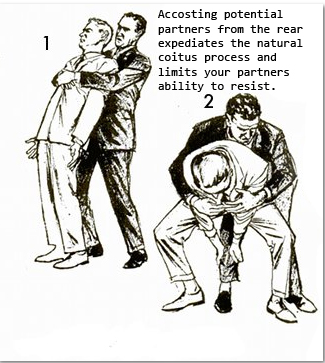
\includegraphics[width=0.4\textwidth]{images/surprise.jpg}
\end{wrapfigure}

Another important part of this section is to convey the mechanisms of overpowering the target. There are not
enough words to capitalize the importance of using excessive restraining measures against the victim. Always
use more force than you may think is necessary while taking care not to overdo it. This is vital because when in
such circumstances the victim's body becomes flooded with adrenaline which makes them significantly more resistant to
pain and much less susceptible to psychological trauma.

\begin{wrapfigure}{r}{0.4\textwidth}
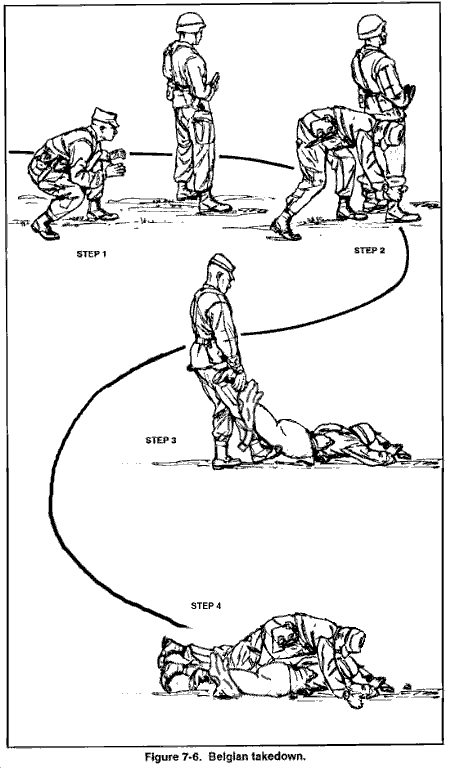
\includegraphics[width=0.4\textwidth]{images/belgian_takedown.png}
\end{wrapfigure}



Do not hesitate to use your fists. A quick slap, or a punch is usually a very effective way to immobilize
the victim for a period between one and five minutes, but take care and exercise caution as to the amount of force
you plan to exert, unless you plan to kill her before starting the natural coitus. Escessive use of punishing 
trauma can visibly disfigure your victim, thus significantly lessening the amount of pleasure you'll derive later 
from your planned activities. However a "perk" of killing her is that she will not need any restraints and getting 
into position is a much easier thing to do. From my own adventures of exploring natural coitus, killing the target
can be highly enjoyable if you can manage to do it cleanly. The body is still warm for a few hours, which is perfect 
for when coitus really gets into its most intense times.



It's also highly reccomended that you use handcuffs against the victim, because it's a relatively efficient,
quick, and easy way to restrain someone while at the same time inducing the maximum amount of fear. The same can
be accomplished with ducktape if necesary, but isn't recommended because it may prove very difficult to tape
someone while she is still actively resisting. Handcuffs click in place immediately and are easier to deploy
in a stressfull situation, making them the utility of choice for your restraining needs.


\begin{wrapfigure}{l}{0cm}
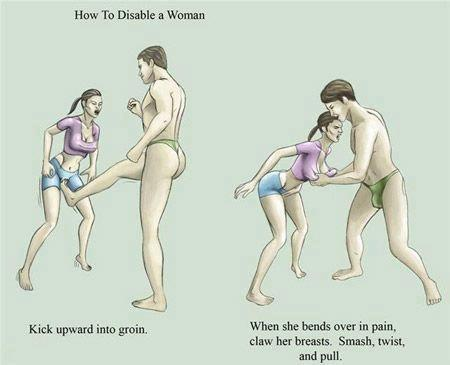
\includegraphics[width=0.5\textwidth]{images/cunt_punt.jpg}
\end{wrapfigure}

Another skill to understand, master, and practice is the ability to silence the prospective rapee.
For this, you may use a sock and duct tape or something similar to block their mouth. 
A gag would also suffice, but make sure you use tape over it or be sure the gag is big enough 
to avoid most of the screaming. However, this step can be skipped if you have the victim in a place of
your choosing you've prepared for just such an occasion. If that is the case, feel free to savor the
auditory bliss associated with the experience. Chains and handcuffs and the like make for poor bindings,
as they allow many degrees of freedom, but the psychological effects simply cannot be beat, and including 
heavy iron chians in your planning can pay off handsomely as they can truly terrify your target. Just make 
sure to avoid suspicision from pesky neighbors while installing the equipment in your basement. 
If they get suspicious, be especially nice to them. This can throw them off as some people will believe that 
"such a nice person wouldn't do that".  If funds allow, consider setting up a full-fledged 'dungeon'. This is 
preferable to enforce intercourse outside, as you have free reign over the victim once you've immobilized and
successfully transported her to your abode. Owning a plot of land in a remote location almost completely
eliminates many of the risks associated with nosy neighbors, wandering postmen, curious
children, and many other such nuisances that could jeopardize your maneuverings. The farther away you are from 
other people, the less likely you are to be found out.

Remember: preparation is half the battle!


\chapter{Evading}

Knowing your terrain is everything for a successful coitus, reading up on
citymaps and or trying to learn the enviornment having a look on various closing times are crucial to a
good rape evasion. Have atleast two escape routes or more when you and your
partner is done with the coitus. Be sure your partner is in a safe location
where he/she can be found, but isn't reachable for random bypassesers for atleast
five minutes or more. Never have coitus outide of your living ground, if you cannot find a remote location
This is highly dangerous and could make your whole coitus all-for-nothing
as you can be recognized by people you may know or a bypasser can easily see.
Another option is having a temporary shelter for the night incase a search
party is set in motion, at that time moving on the streets by foot or car is
not the best idea. Be mindful if the neighborhood is socially close and work
together, or in the big city where people live more anonymously. You must also
have a hiding place, a safe location where you can store various memories and a dumping
place. Do not attempt to keep any evidence of your coitus happenings anywhere near your home.
Do not keep them in your house, someone can, and eventually will find it inside of yor home.
You will also need a place to destroy and clean your rapesuit and rapegear.

Note: Try to not reuse rapegear and rapesuit, unless it is aboslutely detirmental to do so.

\chapter{Social Attitudes Towards Natural Coitus}
\section*{Feminism and the World}

In recent times, the practice of Natural Coitus has come under scrutiny from both the powers that be, and a plethora 
of overzealous individuals who wish it torn asunder simply because it does not mesh with their solipsistic and outdated 
view of morality. This has happened partly because of how Natural Coitus comes across to may people, especially females 
and radical groups such as feminism. Feminism has sunk its jagged claws deep into the very fabric of our society, and, 
as such, commands a large amount of power and influence, especially among the female population and in politics.

Another reason for this rather expected turn of events is because the society of today has become increasingly 
liberal to the point of caricature. The old ways and time-honored traditions of Natural Coitus have becomes 
lost in a maelstrom of degenerate behavior as convervative attitudes have been swept away through decades 
of gradual erosion. The caustic and unnatural worldview that many women hold today directly correlates 
to the rise of feminism, which is itself the bastard child of Cultural Marxism. Both have contributed 
heavily to the infamy and societal persecution of those whose only wish is to practice the natural 
acts of coitus as was the norm in the not-so-distant past of their forefathers.

To illuminate and broaden our understaning of the subject, it must be mentioned that Feminist groups originally 
sprung from the Suffragette movement of the mid to late 1800s, with delusional women from all over Great Britain 
rising up against the superior males of the time. Committing ludicrous acts such as chaining themselves to lamp 
posts (and being general nuisances in order to get their way, much like a child would to persuade their much 
wiser parents to buy them a toy they will soon forget about, and will then move on to wanting something else), 
the women gradually wore down opposition to their cause, and destroyed their detractors piecemeal. The men 
of the time, although well-versed in politics and the social sciences, had little idea of what they were 
up against or the kind of monster it would metamorposize into.

Like tantrum-throwing children, the women marched and demanded their rights, and, in stark contrast to the 
rhetoric of oppression they so actively preach these days, were given everything they demanded. Rights that 
should not have been theirs were granted, concessions made, time-honored traditions trampled, and new laws 
enacted, forcing the carefree male to enfeeble and socially castrate himself in order to fulfill his most 
basic desire for sex (unless said male wished to be jailed for the newly-perpetrated transgressions).

And that indeed is what has happened over the years, with the radical-like feminists standing in the way of 
the processes deemed natural by most experts in gender studies, including myself, along with other professionals 
of similar standing. Natural Coitus is, by itself, simply the process of bringing into the world the next generation 
of great men. It is a natural act, and the stigma associated with it is, from a historal point of view, a recent thing. 
What was natural and widelay accepted only a hundred years ago has now been (to the detriment of us all) relegated to 
the realm of psychopathy.

Today, the Feminist movement is acting much like their Suffragette foremothers - in an extremely aggressive 
manner not befitting the valued, submissive woman. However, despite its long string of victories over the 
course of decades, it is clear the movement has actually lost momentum in recent years. Modern females 
may profess to it when among friends, and even live by its teachings, but, subconsciously, they crave 
the brutal, unyielding dominance of a superior male.

As the old proverb goes, a woman unchained is no woman at all!

The blind solipsism and rabid misandry infecting the Feminists of today keeps them sequestered in a bubble 
of their own making, effectively barring them from realizing these self-evident truths. Women in the 1800s 
were ruled over by men, but they wanted this leadership, *craved* it, for supplication and submission to 
women is what war and natural coitus are to men. It was only when the Suffragettes came along and blinded 
the logical thinking of perfectly well-behaved females that they suddenly came to the radical and silly 
ideas they hold today, namely to involve themselves in things that only men understand and have made 
their spheres of influence since time immemorial. 

Education, finance, politics, law enforcement... all bowed down and opened their doors to the fairer sex, 
admitting women into the chambers of hallowed institutions which had been male-oriented since their inception. 
Even the militaries of the developed world -- those ancient work horses of the nations which had defended their 
people through countless wars -- have, in many countries, allowed females within their ranks.

Nowadays, the Feminist have run out of false oppressions to rail against and equalities to demand, and so 
they dedicate their time and energies to denouncing and shaming those who would otherwise practice the most 
natural of processes, that which has, since the Neanderthals, demonstrated who among a tribe was true Alpha.

First, let us define that word, as done so by Merriam-Webster:
\begin{quote}
 al•pha ('æl fe)
\\
 n., pl. -phas,\\
 adj. n.
\begin{enumerate}
       \item the first letter of the Greek alphabet (A, a).
       \item the first; beginning.
       \item (cap.) the brightest star in a constellation: Alpha Centauri.
       \item the first or foremost in a series of related items. 
\end{enumerate}
 adj.
\begin{enumerate}
\setcounter{enumi}{4}
       \item \begin{enumerate}
          \item  (esp. of animals) having the highest rank of its sex in a dominance hierarchy: the alpha female.
          \item  being the most prominent, talented, or aggressive person in a group: the alpha male of investment bankers.
       \end{enumerate}
       \item pertaining or linked to the carbon atom closest to a particular group in an organic molecule. 
\end{enumerate}
\end{quote}

Now, it has been proven that females prefer the 'Alphas' of society. Ask any Female in the street, and more than 
ninety percent of them will say they prefer a confident, attractive, successful, and well-hung man. This is the most 
widely accept definition of the characteristics which, when they converge in one individual, make him an Alpha male.
Therefore, it is glaringly obvious that women are actually inviting Alphas to plant seeds inside their fertile wombs 
in an effort to secure for themselves and their future progeny the best possible DNA. After all, women are hypergamous, 
and it is socially acceptable (and encouraged) for them to seek the best possible mate, even if they themselves do not 
clome to scratching the upper echelons of female beauty (which is, in all honesty, the only metric of female value).

Returning to our earlier point, the only way of proving who is Alpha is the process of Natural Coitus, for only the 
daring, strong, accomplished, and fearless man posesses the ingenuity and strength of character to attempt Natural 
Coitus at a time of history when all outside variables are pitted against him. In a time when automated labor and 
mechanized warfare have all but replaced the male in fields which had been his proving grounds for untold eons, 
one of the only ways (maybe even the *only* way!) a modern man can demonstrate his value to a female is to rape her. 
This enforces his dominance upon her, and visibly demonstrates his ability to subdue both her mind and her body to 
his will, and at great peril to himself! For, he chances life imprisonment if caught, and the inability to leverage 
his victory over the current female in future conquests even if he succeeds in performing natural coitus without 
sufferring apprehension at the hands of the authorities.

In essence, what once was accepted and even celebrated is now shamed and maligned.

To finally weave all these threads together and put the whole picture into perspective, we must understand one 
final part of the puzzle, and that is the undeniable fact that most females *desire* rape, even if subconsciously. 
However, the majority of disenfranchised males today see feminism as a plague which has robbed them of their God-given
right to practice natural coitus. This, then, leads them to conclusion that feminists, in their fight against Natural 
Coitus, are therefore stopping the human race from progressing, and, as such, should be removed or used for males to 
practice Natural Coitus on. However, while the latter is true, that former is not entirely correct...

Those of us who study female behavior with a critical eye have come to understand that Feminism evolved out of a 
desire to test males. As already mentioned, there are few natural testing grounds left for a man living in the 
relative safety and comfort of the modern world, and the acquisition of wealth, while valuable to a female, does 
nothing to raise a man's status in her eyes if he is not posessed of physical stature, mental power, and dominance. 
And so, Feminism sprung into being, spawned in the darkest recesses of the female mind and nurtured from the 
percolating brine found therein to mature into its final and current form - that which we witness today.

Its *true* purpose is to enforce a life of celibacy for the majority of helpless Beta males, while taunting and 
goading the most capable and ruthless Alphas to defy the law (and common sense) in order to fulfill their need 
for natural coitus. In a way, Feminism is the ultimate mating strategy, as it ensures a win-win scenario for women 
by eliminating the worthless individuals (via proxy, as their own shortocmings consign them to a life of labor and 
self-imposed celibacy) while pushing the worthile to excellence.

It can be said that Feminism is a brilliant, infinitely complex and self-deluding apparatus the female mind has 
enacted in order to receive the rape they crave but eliminate the accompanying shame they do not desire.

Thus, Feminism serves as a mechanism which ennables natural coitus of the highest caliber.

In its purest form, feminism is the vehicle of rape.


\chapter{Overcoming Opposition: The Unenlightened}
During my travels, I have come across many different people and, more importantly, types of people.
Everyone has a preset of opinions -- such is human nature -- and there are always those who militantly
oppose the decisions and lifestyles of others, even when said individuals in no way impact their own
lives or sovereignty. Such narrow-minded people simply cannot be reasoned with. The most efficient
course of action is to simply ignore them, as this causes the least amount of hardship to both them
and yourself.

We as humans must make allowances for the less capable, we are told - a policy drummed into us from a young age.
The idea that your own opinion is 'correct' is often referred to as delusion, and this what I will refer to it
as throughout this chapter.

Now, most human beings assume that their view of the world is the correct one. This is an arrogant assumption
to make as there is no 'right' or 'wrong', merely one's own way. False morality is often used as a hammer to
beat down those who do not conform. Those of us wishing to upset the status quo must resign themselves to
bear the brunt of the ossified legal system, and the wrath of the majority if we are caught furthering mankind
in this way.

As far as opinions go, all are subjective. To bog oneself down in endless moral dilemmas is to purposefully
ignore the joys of living free and claiming for yourself what nature has rightfully bestowed upon you. Human
interactions are often characterized by dominance, and natural hierarchies are just that; natural. This is
true for both the micro and macro-level strata of human civilization.

Delusion comes in many forms, however the most dangerous one is aggression. An emotion widely used by
feminists to fuel their many smear campaigns, it is the driving force of all delusion within the feminist
regimes. They feed on it like maggots on rotting flesh, and it empowers them in their crusades against the
stronger, more noble sex. It is important I stress the link between delusion and feminists, as that is at
the very core their zealous religion.

A topic raised time and again by feminists everywhere is Natural Coitus, however they are usually portraying
a skewed, exaggerated, or a downright untruthful version of it, claiming the Natural Coitus is actually
harmful to females and the female 'race' of 'womyn' as a whole.

Nothing could be further from the truth.

When tackling with these feminists it is extremely important to treat them with a degree of sympathy, as
feminism itself is a well-known mental disorder. Those poor souls, in their neverending and joyless quest
to usurp from man his rightful place, know not the ecstatic bliss they so foolishly disregard in order
to chase after unnatainable goals and insatiable appetites of the most material sort.

A woman's whole existance revolves around subjugation. She is a vessel of the man's seed, and it is her
divine duty to submit to a strong man. Her place is at his feet, chained to his fate by his own iron will,
and ready to service him in any and all ways he wishes. Modern feminism long ago abandoned these sacred
tenants of the age-old covenant. As a result, their foolishness has wreaked havoc on the whole of society.

Women, being the limited creatures that they are, cannot accept that Natural Coitus is, and always has been,
a process of demonstrating the natural hierarchy within a society. This simple fact is demonstrated time and
again by animals in the wild. One example would be bears, who perform Natural Coitus quite often, and to such
an extent that it is seen as completely acceptable so long as the Male bear has already asserted its dominance.

If approached by a feminist, it is often regarded a necessity that you immediately proclaim the following
words, 'Natural Coitus is the way of the world'. This demonstrates you are enlightened to a higher level of
understanding, and as a result you are actually of a higher social status and are fundamentally a better
person than they are. Usually this unsettles even the most hardened of feminists.

If this approach doesn't work it is best to retreat to a pre-arranged tactical location and avoid contact,
as feminists, once pushed, can rarely be reasoned with. Then again, they make prime Coitus candidates, as 
their very nature belies weak women who yearn for a strong male figure to come into their lives and 
literally sex them into submission. Explaining this to them is almost impossible, which is why, in
the case at least, words should give way to deeds.



\chapter{Safe Alternatives}
 
Has the act of raping other humans become monotonous, and the effort of leaving 
your home become too much? If so, this chapter is definitely worth looking into. 
Followed correctly, this simple manual will show you different methods of rape 
that can be a safe and fun alternative to raping women or children, and it will 
show how such acts can be productive and informative. Written by the 
critically-acclaimed author James B. Rustles, this short manual contains several 
surefire methods to feeding your desire to rape, while staying in the legal 
realms of the law.


\section*{Solution 1: SELF-RAPE}

While some may doubt this alternative to rape, it has been proven that self-rape 
is a great way to curb your appetite for rape, and can result in an amazing 
self-bonding experience with ones body only achievable by means of self-rape.

1) Treat yourself to a few drinks or other soft drugs that are available or near 
your location; loosen up a bit and relax a little. Turn on the TV, radio, or 
just lie down on the couch. Make sure you get in a comfortable and relaxed 
state.

2) If things are already going well and you’re feeling about to pass out, 
continue, but if not, you may need some extra help. In this case throw half a 
roofie tablet into the drink when you’re not looking, and then continue to drink 
at a comfortable pace.

3) From here it's incredibly easy to take advantage of your unsuspecting self. 
Simply take off your pants (by force if necessary).

4) Slide your hand onto your penis. It should be erect by now. Stroke your penis 
slowly, but firmly and increase the pace as you go. Slide a couple fingers into 
your asshole, sodomy is historically a key part in self-rape and is still 
relevant today. (Note: it may hurt momentarily, but you will experience pleasure 
after your asshole gets accustomed to it.)

5) You’ll know when you have been successful if a milky white liquid erupts from 
the tip. This liquid is called semen. As appetizing as this liquid may seem, it 
is not recommended you ingest it, however there are no health risks involved in 
doing so.


Other various methods of self-rape include but are not limited to:


    Leaving a plunger in the toilet and sitting on it when you go to use the 
restroom (A.K.A. The Hellen Keller). (This method may result in death or serious 
colon injury.)


    Sticking a suction cup phallus shaped object on a chair and leaving it there 
until you sit on it (this method is known to be slightly uncomfortable, however 
is still a healthy and widely used method).


    Obtaining a life-size poster of your naked backside with an appropriately 
positioned anal cavity can simulate self-rape to a certain degree.


    Placing a vacuum cleaner hose around your erect penis.  From here simply 
turning on the aforementioned vacuum can produce rape-like sensations.



\section*{Solution 2: RAPING INANIMATE OBJECTS}

Raping inanimate objects result with no legal repercussions and no life changing 
consequences. In Afghanistan, it's very common to make love to sand dunes before 
you make love to a woman. It is also common for young boys to make insertions 
into their bed to insert their penis into the tight hole of the fabric. Some 
inanimate objects


Steps to a common method of the rape of inanimate objects:


1) Open a door until there is a certain amount of room to diligently put your 
penis in the remaining space. this will give pleasure as it simulates sexual 
activity to the shaft and tip of the penis.


\chapter{Hints, Tips, Extras}
\section*{The look:}
The look plays a big role in the process of negotiation. You have to make sure that you're looking your partner in the eye, in order to make them feel comfortable and earn their trust. Try not to look angry or in a hurry, as this may be considered offensive in some cultures.
Your smile will also affect the emotional state of your partner, a warm smile with no teeth showing gives the best results, according to a German research team specializing on the effects of smiling at various species of animals.

\section*{The location :}
A friend of mine, Steve Robtorn, also a writer, once said: "Not every place is a good place." You have to choose wisely the place of your partner’s dream, and drag them into it. Use a blindfold on the way there to make it a cute surprise.

\section*{The time :}
Many men are too rushed, they try to end it as quickly as they can for fear of being noticed. This is wrong and insensitive! Your partner is enjoying it, no matter what they may be screaming to the contrary, and you need to make it last as long as you can. Try not to be selfish as this will ruin your partner’s enjoyment and that not what you want to do. Try moving your partner to multiple locations, using various methods of transportation (such as the trunk of a car). This will make it seem to last forever, and is key to achieving natural coitus.

\section*{The manner :}
We discussed above the time and we have to talk about the manner too. "Hard" is the word that should be floating in your heading in the time of the execution. A recent online poll from Jezebel.com showed that 97.8 percent of partners like it rough and hard, all the while denying this and yelling that they want out. The more you hear the word "stop", the more they want you to keep going. Who are you to leave their innermost desires unsatisfied?



% Last pages for ToC
%-------------------------------------------------------------------------------
\newpage
% Include dots between chapter name and page number
\renewcommand{\cftchapdotsep}{\cftdotsep}
%Finally, include the ToC
\tableofcontents




\end{document}

